\chapter{双频激光干涉仪的环境误差及Edlen公式补偿方法}




\section{激光位移测量理论基础}
目前许多常见的激光位移测量方法,其原理大多基于多普勒频移,将位移/速度变化转变为信号的相位变化进行测量;同时为了提高测量精度,并且减小低频噪声的干扰,往往利用拍频现象,将测量信息挂载在两个波叠加产生的拍上,其幅值是随着时间周期变化的,从而将测量信号从直流量转变为交流量。



\subsection{多普勒频移}
多普勒频移(Doppler Shift)是由奥地利科学家Christian Johann Doppler于19世纪发现提出的\cite{基于激光多普勒测速的自由场空气声压测量研究},该效应指的是当接收体与波源之间存在相对运动时,接收体接收到的波的频率与波源发出的频率不相同,并在波源本身频率的基础上发生了一定的频移,即为多普勒频移。

多普勒频移的产生是由于运动导致波的传播路程差发生了变化,使得波对于接收体而言在空间中不是均匀分布了,如图\ref{fig:多普勒频移示意图}所示,当波源位置从S1变为S2时,接收体所在的P点单位时间内接受到的波的个数增加,即接收体处的波的频率增加,反之则频率减小。一般性的,当波源和接收体相互靠近时,波被压缩,接收体单位时间内接收到的波的个数增加,即频率变高;当波源和接收体相互远离时,波被拓展,接收体单位时间内接收到的波的个数减少,即频率变低。
\begin{figure}[htb]
    \centering
    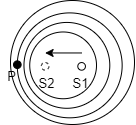
\includegraphics[width=3.5cm]{fig/2-fig/多普勒频移示意图.png}
    \caption{多普勒频移示意图}
    \label{fig:多普勒频移示意图}
  \end{figure}

由于波源和接收体之间的相对运动而产生的频率变化值的大小与相对运动的速度之间存在定量推导关系,从而使得多普勒频移广泛应用于激光速度/位移测量领域。如图\ref{fig:多普勒频测速示意图}所示,接收体处在\(P\)点,波源从点\(S1\)以速度\(v\)朝着点\(S2\)运动时,有:
\begin{equation}\label{eq:多普勒频测速原理1}
    \Delta L=dcos\theta=v\Delta tcos\theta.
\end{equation}
\begin{figure}[htb]
    \centering
    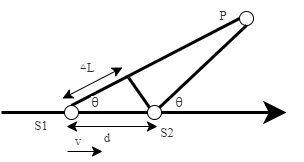
\includegraphics[width=8cm]{fig/2-fig/多普勒频测速示意图.drawio.png}
    \caption{多普勒频测速示意图}
    \label{fig:多普勒频测速示意图}
  \end{figure}

式\eqref{eq:多普勒频测速原理1}中\(\theta\)是\(S1\)和\(S2\)处出射波的夹角,\(\Delta L\)两处位置的波程差,\(\Delta t\)为运动所需的时间。由于在实际测量中,波源或者接收体在单位时间内运动距离相比于波源和接收体之间的距离很小,所以可以近似认为\(S1\)和\(S2\)两处的\(\theta\)是相同的\cite{百度百科-多普勒频移},由于波的传播路程差导致的相位变化值为:
\begin{equation}\label{eq:多普勒频测速原理2}
    \varphi=\frac{2\pi \Delta L}{\lambda}=\frac{2\pi v\Delta t}{\lambda}cos\theta.
\end{equation}

对式\eqref{eq:多普勒频测速原理2}左边进行变换,即可得到多普勒频移与运动速度v之间的关系:

\begin{equation}\label{eq:多普勒频测速原理3}
    \varphi_d=\frac{\Delta varphi}{2\pi \Delta t}=\frac{v}{\lambda}cos\theta.
\end{equation}



\subsection{拍频现象}
对于两个振动方向相同、振动频率相同并且相位差恒定的简谐波叠加,会在空间中产生强弱相间的固定分布,这种现象称为干涉。如若两个简谐波的振动频率略有差异,其叠加时会在空间中产生幅值随时间变化的周期性分布,这种现象则称为拍\cite{基于拍频测量温度和旋光角的方法研究},拍频则定义为单位时间内合振幅周期性强弱变化的次数。

假设两个振动方向相同的简谐波的方程为
\begin{equation}\label{eq:简谐波方程1}
    x_1=A_1cos\omega_1t.
\end{equation}
\begin{equation}\label{eq:简谐波方程2}
    x_2=A_2cos\omega_2t.
\end{equation}

上式中\(A_1=A_2\),并且\(|\omega_1-\omega_2|<<\omega_1+\omega2\),那么\(x_1\)和\(x_2\)在空间中相遇叠加产生的拍的方程为:
\begin{equation}\label{eq:简谐波叠加后方程}
   x=x_1+x_2=2Acos(\frac{\omega_2-\omega_1}{2}t)cos(\frac{\omega_2+\omega_1}{2}t).
\end{equation}

\begin{figure}[htb]
    \centering
    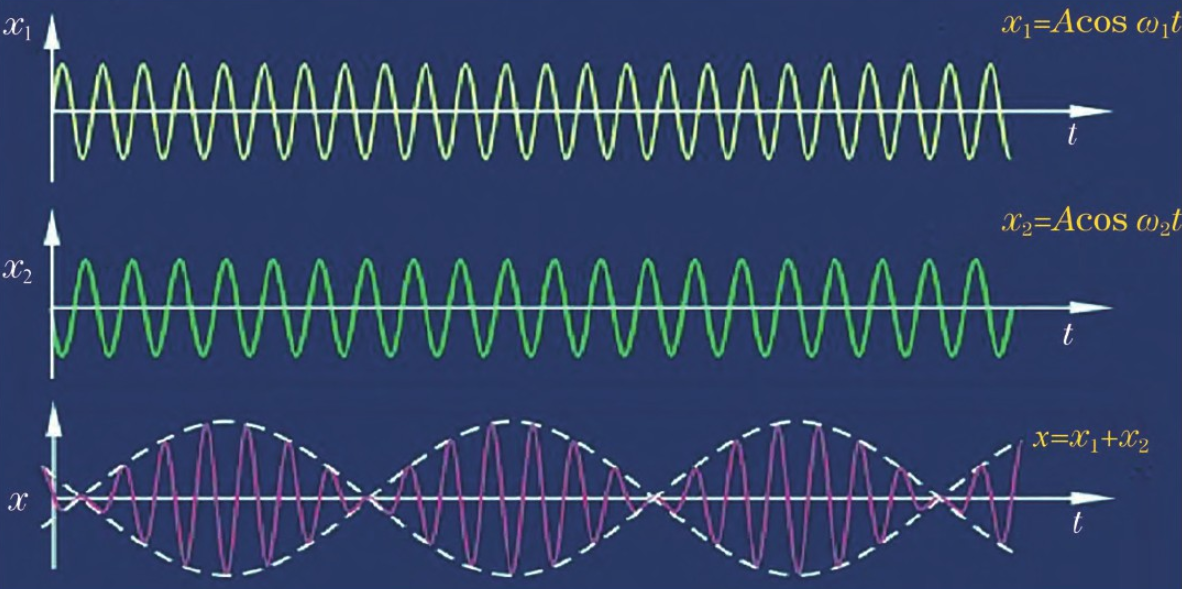
\includegraphics[width=10cm]{fig/2-fig/拍频波形示意图.jpg}
    \caption{拍频波形示意图\cite{激光外差干涉技术在光刻机中的应用}}
    \label{fig:拍频波形示意图}
    \end{figure}
上式中\(|2Acos(\frac{\omega_2-\omega_1}{2}t)|\)为\(x_1\)和\(x_2\)在空间中叠加后拍的幅值,可以看出这是一个随时间周期性变化的值,而\(\frac{\omega_2+\omega_1}{2}\)则为拍的角频率,这也是一个随着时间周期性变化的值,两者共同导致了拍在波形上表现为周期性变化的形式,如图\ref{fig:拍频波形示意图}所示。

并且由式\eqref{eq:简谐波叠加后方程}可以看出,拍的频率为两个简谐波的原始频率之差,虽然当前激光的频率通常很高(约为\(10^{14}Hz\)量级),这使得目前的光电探测器无法响应\cite{激光外差干涉技术在光刻机中的应用},但通过拍频现象,即可将高频的信息转变为低频信息,便于光电探测器响应。



\section{激光干涉仪原理}
\subsection{单频激光干涉仪}
单频激光干涉仪,也可以称为零差干涉仪,具有精度高、稳定可靠, 且相对成本较低等特点\cite{零差干涉仪用于振动校准中关键技术的研究}。其示意图如图\ref{fig:单频激光干涉仪原理图}所示。
\begin{figure}[htb]
    \centering
    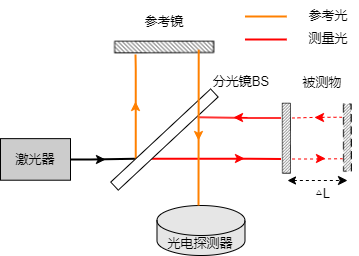
\includegraphics[width=7cm]{fig/2-fig/单频激光干涉仪原理图.drawio.png}
    \caption{单频激光干涉仪原理图}
    \label{fig:单频激光干涉仪原理图}
\end{figure}

激光器出射的激光经过分光镜BS后产生两束光:一束进入参考臂,并被参考镜反射,另一束进入测量臂,并被被测物体反射,当被测物体位移为\(\Delta L\)时,测量光会携带上对应的多普勒频移\(f_d\),两束光分别经参考镜和被测物体反射后会再次汇聚,随后射入光电探测器,根据相位的变化即可反推被测物体的位移。

\subsection{双频激光干涉仪}
双频激光干涉仪结构如图\ref{fig:双频激光干涉仪原理图}所示,激光出射的含有\(f_1\)和\(f_2\)两个频率成分的激光经过偏振分光棱镜(polarization beam splitter,PBS)分为测量光\(f_1\)和参考光\(f_2\),测量光\(f_1\)进入测量臂之后,携带上被测物体位移\(\Delta L\)的多普勒频移\(\Delta f\)。由于测量臂和参考臂上各放置了一块四分之一玻片(Quarter Wave Plate,QWB),测量光和参考光在返回PBS之前都经过两次QWB,使得其偏振态发生改变,原本透射的测量光再次返回PBS时变为反射,原本反射的参考光再次返回PBS时变为透射,参考光和测量光汇聚,耦合进光纤,由采集板卡从多普勒频移\(\Delta f\)解调出被测物体的位移\(\Delta L\)。
\begin{figure}[htb]
    \centering
    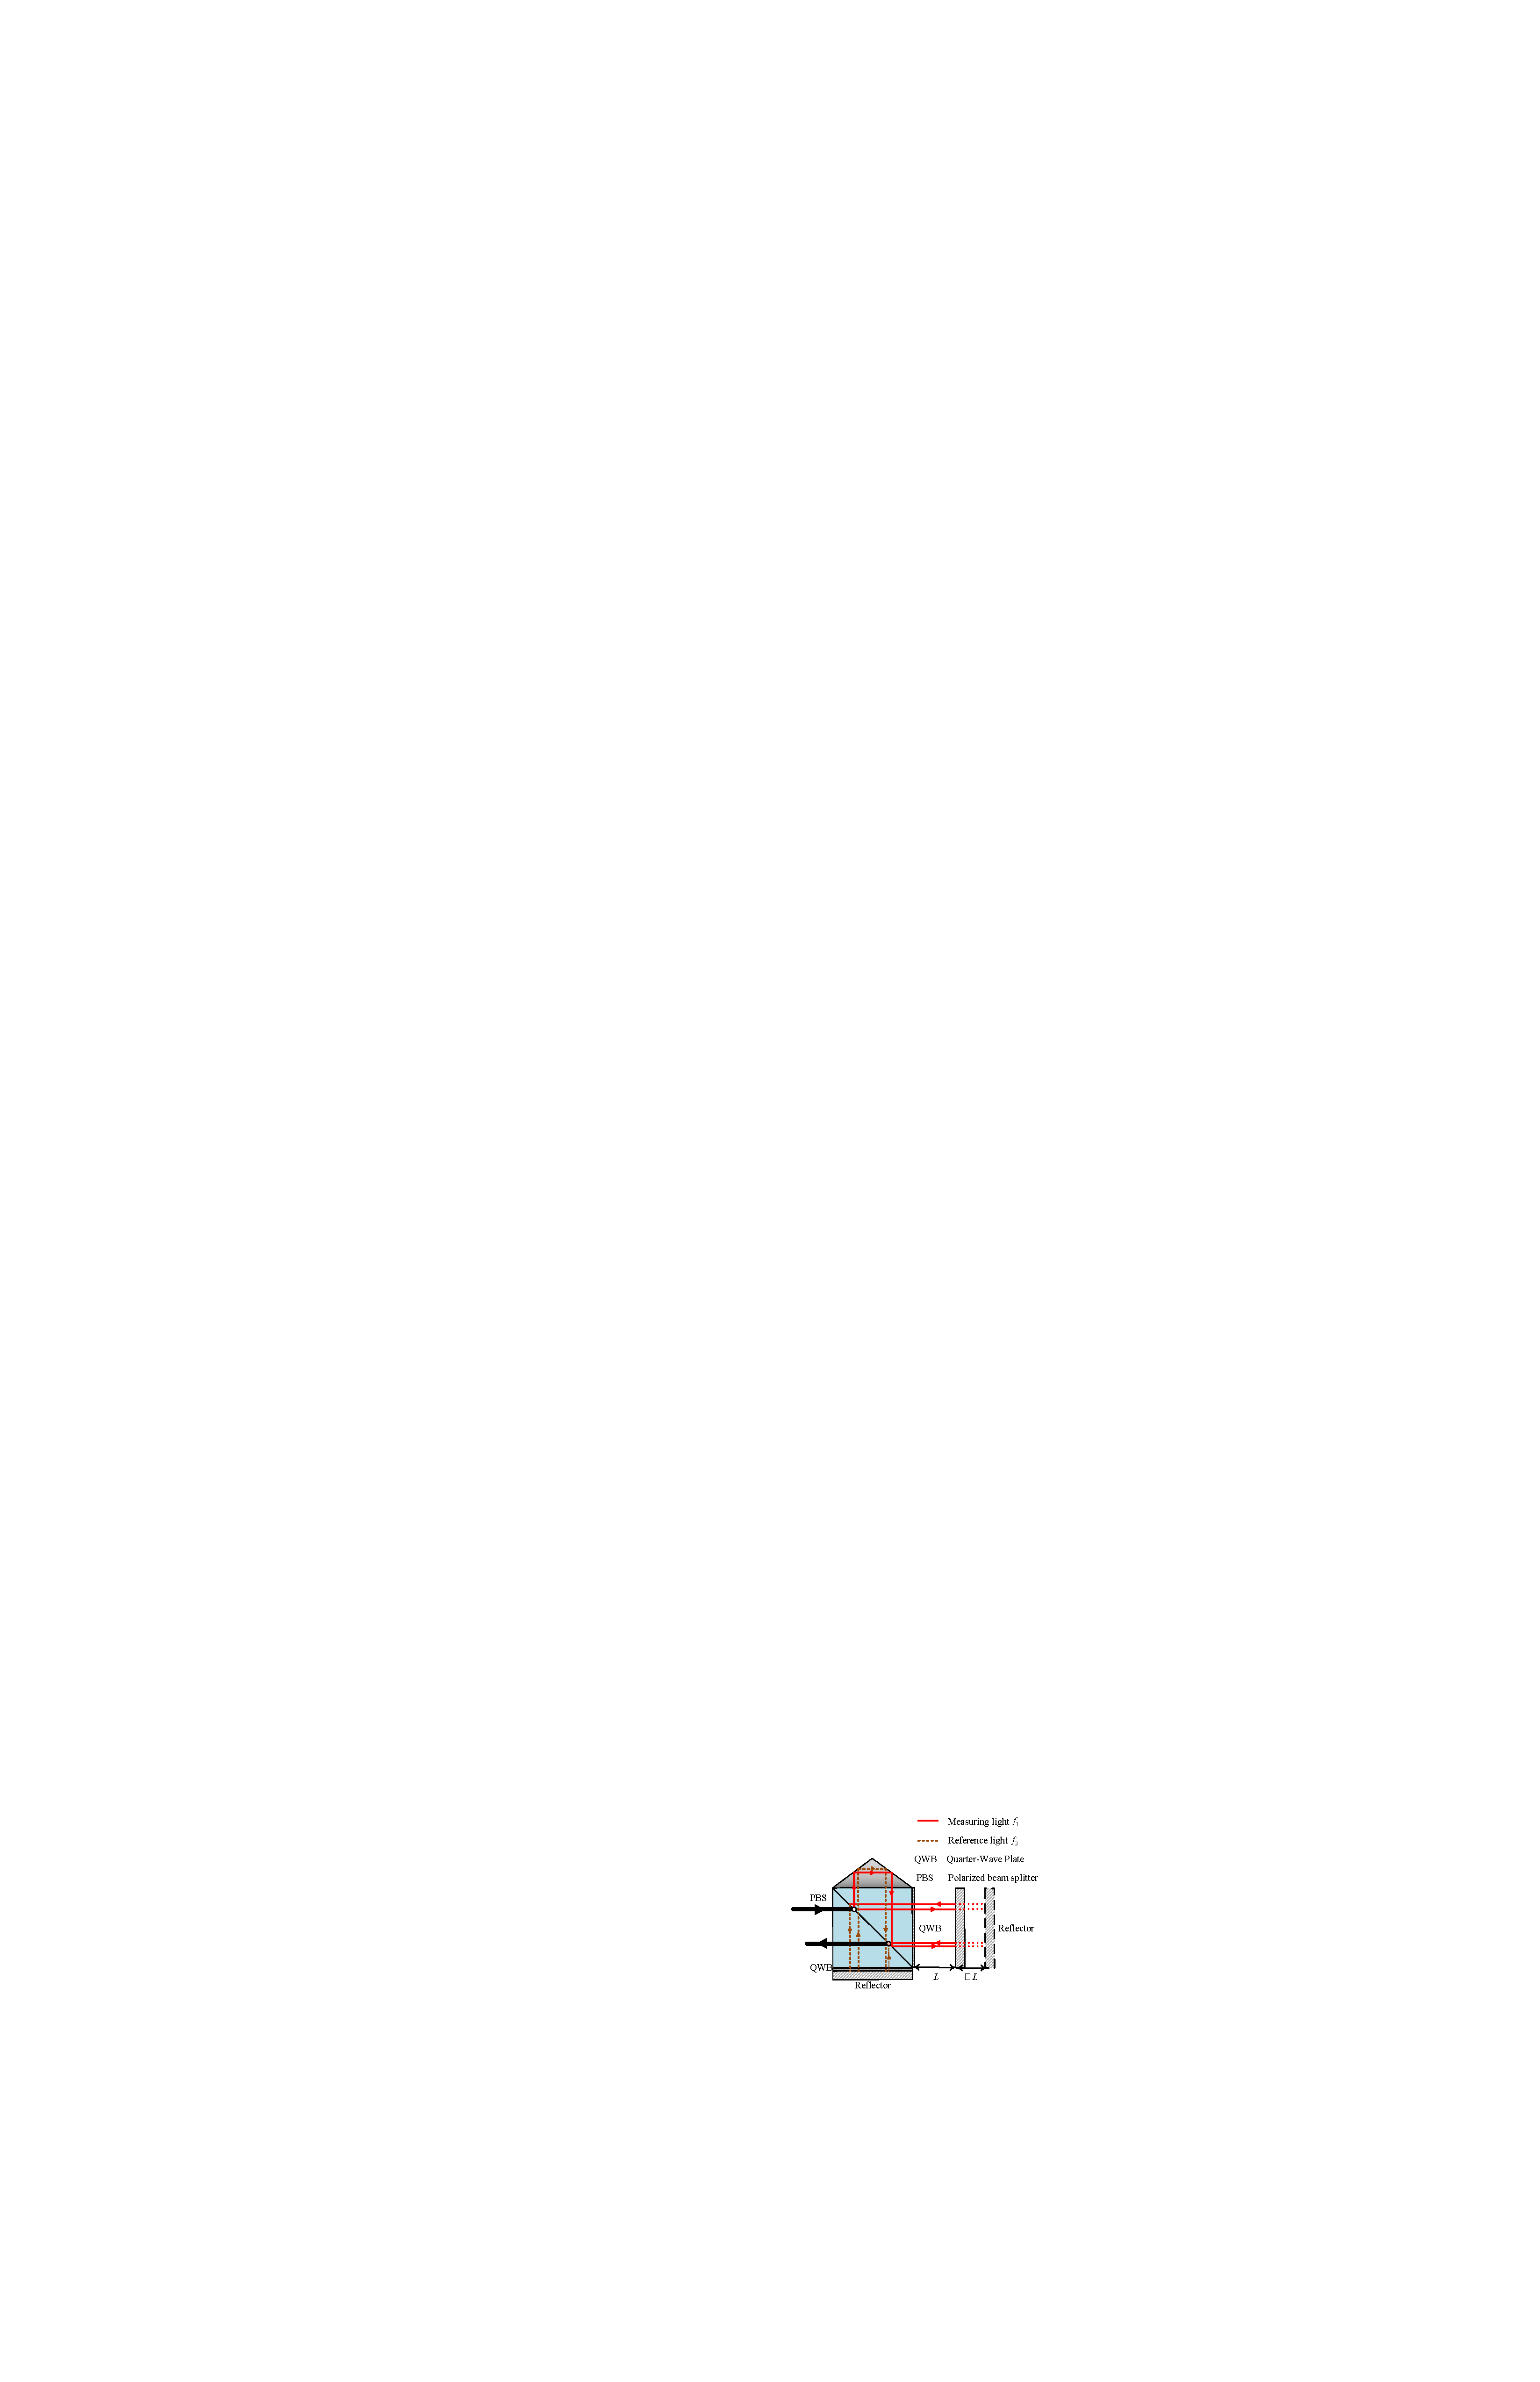
\includegraphics[width=8cm]{fig/2-fig/双频激光干涉仪原理图.pdf}
    \caption{双频激光干涉仪原理图}
    \label{fig:双频激光干涉仪原理图}
\end{figure}

\section{双频激光干涉仪的环境误差及其成因}
在实际的测量当中,测量值\(D\)是指干涉仪系统实际输出的位移值。是由条纹数\(N\)乘上干涉仪系统的分辨率\(R_{es}\)得到的,而条纹数\(N\)与光程的变化有光,即:
\begin{equation}\label{eq:测量值与光程的关系}
    D=R_{es}{\times}N=R_{es}{\times}\frac{\Delta L{\times}n_0{\times}M_o}{\lambda{\div}M_e}=\Delta L{\times}n_0.
\end{equation}

式\eqref{eq:测量值与光程的关系}中,\(n_0\)为真空中的空气折射率,近似可认为1,分辨率\(R_{es}\)与激光的实际波长\(\lambda\)、电子细分\(M_e\)和光学细分\(M_o\)有关。电子细分\(M_e\)由采集办卡决定,常见的有32、64、128……2048等,而光学细分\(M_o\)与干涉仪的设计结构有关,具体计算公式如下:
\begin{equation}\label{eq:分辨率与细分的关系}
    R_{es}=\frac{\lambda}{M_o{\times}M_e}.
\end{equation}

当外界环境因素(温度、气压等)变化导致空气折射率变化\(\Delta n\)时,干涉仪系统测量值\(D\)不仅包括被测物体的位移\(\Delta L\),还包括由于折射率变化引起的光程变化\(\Delta l\),即:
\begin{equation}\label{eq:实际的位移公式}
    D=\Delta L(\Delta n+n_0)+L\Delta n.
\end{equation}

由于测量臂长度\(L\)一般远大于被测物体位移\(\Delta L\),由式\eqref{eq:测量值与光程的关系}和式\eqref{eq:实际的位移公式}可得,由于外界环境因素(温度、气压等)引起的误差为:
\begin{equation}\label{eq:环境误差公式}
    D=[\Delta L(\Delta n+n_0)+L\Delta n]-\Delta Ln_0=\Delta n(\Delta L+l) \approx \Delta n \Delta L.
\end{equation}



